\documentclass{article}

\usepackage{amsthm}
\usepackage{amsmath}
\usepackage{amsfonts}
\usepackage[margin=0.5in]{geometry}
\usepackage{hyperref}
\usepackage{tikz}
\usepackage{wasysym}

\DeclareMathOperator{\re}{re}
\DeclareMathOperator{\res}{res}


\title{\href{https://math.umn.edu/sites/math.umn.edu/files/exams/complexs19.pdf}{Spring 2019 Complex Analysis Preliminary Exam}}
\author{University of Minnesota}
\date{}
\begin{document}
\maketitle


\begin{enumerate}
	\item Give a conformal mapping from the (open) upper half plane to the slit disk \[ D = \{ z \in \mathbb{C} : |z| < 1, z \not \in [0,1] \}\]
	
	% See PG notes 3.0.3. We are looking for the inverse of the Cayley map.
	% The Cayley transformation according to Wikipedia is the inverse of the Cayley map according to PG
	% See also Mobius transformation which PG calls a fractional linear transform.
	\begin{proof}
		Consider the map $f(z) = \frac{z-i}{z+1}: \mathbb{C} \rightarrow \mathbb{C}$. Note that this is a fractional linear transformation.
		
		Let $H$ be the open upper half plane.
		We first want to show that $f(H) = D$.
		
		First, when we restrict $f$ to the real line, we see $\lim_{x \rightarrow \pm \infty} f(x) = 1$. We also see that 
		\begin{align*}
			f(1) &= \frac{1-i}{1+i}\\
				&= \frac{(1-i)^2}{ | 1+i|^2}\\
				&= \frac{1-2i-1}{ (\sqrt{2})^2}\\
				&= -2i/2 \\
				&= -i
		\end{align*}
		and
		\begin{align*}
			f(-1) &= \frac{-1-i}{-1+i}\\
				&= \frac{(-1-i)^2}{|-1+i|^2}\\
				&= \frac{1 + 2i - 1}{ (\sqrt{2})^2 }\\
				&= +i
		\end{align*}
		finally
		\[f(+i) = \frac{i - i }{i+i} = 0.\]
		Thus, because fractional linear transformations preserve circles-and-lines, and $+i \in H$ gets mapped to the interior of $D$, then $f(H) = D$.

		Now we show that $f(z)$ is conformal on the open upper half plane. $f$ is conformal where its derivative is nonzero, and so we compute
		$f^\prime = \frac{(z+1)- (z-i)}{(z+1)^2} = \frac{1-i}{(z+1)^2}$, which is defined except at $z=-1$ (which is not in the open upper half plane so we need not worry) and is nonzero wherever it is defined.
		Thus, $f$ is a conformal mapping from $H$ to $D$.
		 
	\end{proof}
	
	\newpage
	
	\item Write the first three terms of the Laurent expansion of $\displaystyle f(z) = \frac{1}{z^5-1}$ centered at $0$ and convergent in $|z|<1$.
	
	\begin{proof}
		Observe that \[\frac{1}{z^5-1} = \frac{-1}{1-z^5} = -\sum_{n=0}^\infty z^{5n}\]
		which converges for $|z^5|<1$ which is $|z|^5<1$ or $|z|<1$. 
		Thus, the first three nonzero terms of the expansion of $f$ are 
		$a_0 = -1$, $a_5=-1$, and $a_{10} = -1$.
	\end{proof}
	
	\item Classify entire functions $f$ such that $|f(z)| \leq 1 + \sqrt{|z|}$
	
	\begin{proof}
		We appeal to Cauchy's inequality which states that if $f$ is entire, and $\gamma_R$ is any
		circle of radius $R$ centered at the origin, then 
		\[ |f^{(n)}(0) | \leq \frac{n! \sup_{z \in \gamma_R} f(z)}{R^n}.\]
		Since $f$ is entire, pick a power series representation centered at $0$, and call it 
		$f(z) =: \sum_{n \geq 0} \alpha_n z^n$.
		Then $\alpha_n = \frac{f^{(n)}(0)}{n!}$, and so
		\begin{align*}
		| \alpha_n | & \leq \frac{\sup_{z \in \gamma_R} f(z)}{R^n} &\text{(By Cauchy's ineq.)}\\
		&\leq \frac{ \sup_{z \in \gamma_R} (1+ \sqrt{|z|})}{R^n} &\text{(Bound provided)}\\
		&=\frac{1 + \sqrt{R}}{R^n} & \text{($|z|$ is constant on $\gamma_R$)}.
		\end{align*}
		Since this must hold for all $R$ and all $n$, we take the limit
		\[|\alpha_n| \leq \lim_{R \rightarrow \infty} \frac{1+\sqrt{R}}{R^n} = \begin{cases} 0 & n \geq 1 \\ \infty & n = 0 \end{cases}\]
		which forces $f$ to be a constant function.
		Note now that if $f$ is constant, then $f(z) = f(0)$ for all $z$, and so the provided bound that
		$|f(z)| \leq 1 + \sqrt{|z|}$ tells us that $|f(z)| \leq 1$. So we conclude that $f(z)$ is a constant function taking a 
		value inside the unit disk.
	\end{proof}
	
	\item Evaluate $\displaystyle \int_{-\infty}^\infty \frac{\sin(x)}{1+x^2} dx$
	
	\begin{proof}
		Let $f: \mathbb{C} \rightarrow \mathbb{C}$ be given by $f(z) = \frac{-i e^{iz}}{1+z^2}.$ 
		When we restrict to $x \in \mathbb{R}$, we have 
		$f(x) = \frac{-ie^{ix}}{1+z^2} = \frac{-i(\cos x + i \sin x)}{(z+i)(z-i)}$ and so $f$ has real part $\re f(x) = \frac{\sin(x)}{1+x^2}$.
		Thus, the real part of the integral $\re \left (\int_{-\infty}^{\infty} f(z) dz \right)$ is the integral we wish to compute.
		
		Note that the numerator of $f$ is entire and the denominator is also entire and is only $0$ at $z = \pm i$.
		
		Let $t>0$ and let $\gamma_t$ be the curve given by the union of $[-t,t] \subset \mathbb{R}\subset \mathbb{C}$ with the upper half-circle of radius $t$, with positive orientation. 
		Visually:
		\begin{center}
		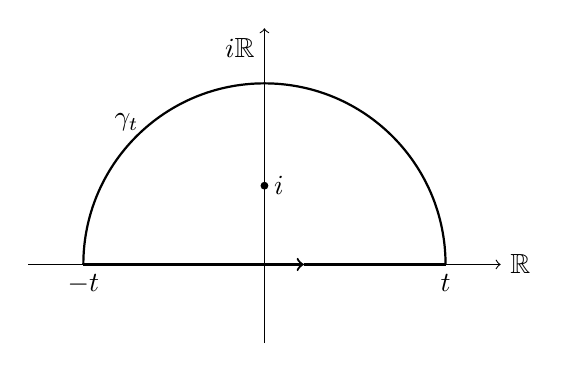
\begin{tikzpicture}
			%\draw[step=1cm,gray,very thin] (-2.9,-0.9) grid (2.9,2.9);
			\draw[thin,->] (0,-1) -- (0,3); 
			\draw[thin,->] (-3,0) -- (3,0);
			
			\node[anchor = north east] at (0,3) {$i \mathbb{R}$};
			\node[anchor = west] at (3,0) {$ \mathbb{R}$};
			
			\node[fill = black, inner sep=1pt, circle] at (0,1) {};
			\node[anchor = west] at (0,1) {$i$};
			
			\node[anchor = north] at (2.3,0) {$t$};
			\node[anchor = north] at (-2.3,0) {$-t$};
			
			\node at (-1.75,1.8) {$\gamma_t$};
			
			\draw[thick] (2.3,0) arc (0:180:2.3) ;
			\draw[thick,->] (-2.3,0) -- (0.5,0) ; 
			\draw[thick] (0.5,0)--(2.3,0);
		\end{tikzpicture}
		\end{center}
		
		Since $f$ is holomorphic on and inside $\gamma_t$ except at $i$, which is a simple pole
		the residue theorem tells us that 
		$\int_{\gamma_t} f(z) dz = 2\pi i \res_{i} f(z)$.
		
		To compute $\res_i f(z)$, take $\lim_{z \rightarrow i} (z-i) f(z) = \lim_{z \rightarrow i} \frac{-ie^{iz}}{z+i} = \frac{-i}{e (2i)} =\frac{-1}{2e}$
		
		So then $\int_{\gamma_t} f(z)dz = -\frac{\pi i}{e}$.
		
		We can split the integral into the part along $[-t,t]$ and along $C_t$, the upper half-circle of radius $t$, as
		\[ \int_{\gamma_t} f(z) dz = \int_{[-t,t]} f(z) dz + \int_{C_t} f(z) dz.\]
		We can use the estimation lemma to bound the magnitude of integral over the half-circle as 
		\begin{align*}
			|\int_{C_t} f(z) dz |&\leq \pi t \sup_{z \in C_t} |f(z)|.
		\end{align*}
		To compute 
		\begin{align*}
			\sup_{z \in C_t} |f(z)| &= \sup_{z \in C_t} \left | \frac{-ie^{iz} }{1+z^2} \right |\\
			&= \sup_{z \in C_t} \frac{|e^{iz} |}{|1+z^2|} \\
		\end{align*}
		When we consider $z = x+iy \in C_t$, we see that $|e^{iz}| = |e^{i(x+iy)}| = | e^{ix-y} | = e^{-y} \leq 1$
		so 
		\begin{align*}
			\sup_{z \in C_t} \frac{|e^{iz} |}{|1+z^2|} & \leq \sup_{z \in C_t} \frac{1}{|1+z^2|} \\
			&\leq \sup_{z \in C_t} \frac{1}{||z^2|- |-1||} & (\text{reverse triangle inequality})\\
			&= \sup_{z \in C_t} \frac{1}{| |z^2| - 1|}\\
			&= \sup_{z \in C_t} \frac{1}{| t^2 -1 |}\\
			&= \frac{1}{|t^2-1|}.
		\end{align*}
		
		Thus, we have
		\[ \left |\int_{C_t} f(z) dz \right |\leq \pi t \frac{1}{|t^2-1|}  \]
		and taking the limit $t \rightarrow \infty$ we see
		\[ \lim_{t \rightarrow \infty} \int_{C_t} f(z) dz = 0.\]
		Thus, in the limit
		\[ \lim_{t \rightarrow \infty} \int_{\gamma_t} f(z) dz = \lim_{t \rightarrow \infty} \int_{[-t,t]} f(z) dz = \int_\mathbb{R} f(z) dz.\]
		The integral over $\gamma_t$ was independent of $t$ (thanks residue theorem \smiley{}), so we see
		\[ \int_\mathbb{R} f(z) dz = \frac{-\pi i}{e}.\]
		We wanted to compute the real part
		\[ \int_\mathbb{R} \frac{\sin x}{1+x^2} dx = 0.\]
		
		We could also see that $1+x^2$ is an even function and $\sin(x)$ is an odd function so $\sin(x)/(1+x^2)$ is an odd function, 
		so its integral must be 0, but why do that when we could use the residue theorem \smiley{}.
	\end{proof}	
	
	\setcounter{enumi}{4}
	
	\item Determine the radius of convergence for the power series of $\sqrt{z}$ at $z_0 = -3 + 4i$.
	
	\begin{proof}
	The radius of convergence of the power series of $\sqrt{z}$ is the radius of the largest disk for which there is a holomorphic function which agrees with $\sqrt{z}$.
	%
	Recall that we define complex exponentiation by $z^\alpha := e^{\alpha \log z}$, so $\sqrt{z} = e^{\log(z)/2}$. Composition of holomorphic functions is holomorphic, so since $e^w$ is entire, the radius of convergence is limited by $\log(z)$. 
	
	There is no number $w \in \mathbb{C}$ such that $e^w = 0$, and so there is no possible way to have a holomorphic logarithm at $0$. This bounds the radius of convergence from above by $|-3 + 4i - 0|=5$. 
	
	On the other hand, it is a theorem\footnote{Theorem 6.1 in Chapter 3 of Stein and Shakarchi's \textit{Complex Analysis}} that if $\Omega$ is simply connected and does not contain $0$, then there is a branch of the logarithm which is holomorphic on $\Omega$. Consider the open disk $D$ of radius $5$ and centered at $-3 + 4i$. Clearly $D$ does not contain $0$, and so there is a logarithm (call it $\log_D$) which is holomorphic on $D$. Thus, we have a disk of radius $5$ on which there is a holomorphic function $\log_D$ which agrees with $\log$, and so the radius of convergence is \textit{at least} 5. 
	
	Since we know the radius of convergence is both at least 5 and less than or equal to 5, we see that the radius of convergence of the power series for $\log$ is in fact $5$.
	
	\end{proof}
	
	\item Let $f,g$ be holomorphic functions on $\{z : |z| < 2\}$ with $f$ nonvanishing on $|z| = 1$. Show that for all sufficiently small $\epsilon>0$ the function $f+ \epsilon g$ has the same number of zeros inside $|z| = 1$ as does $f$. 
	
	\begin{proof}
		Since $f,g$ are holomorphic on $\{ z: |z| < 2\}$, they are holomorphic on the compact sets $D = \{z : |z | \leq 1\}$ and its boundary $\partial D =\{z : |z| = 1\}$.
		
		Rouche's theorem states that if $|\epsilon g| \leq |f|$ on $\partial D$ (which can be thought of as a closed curve) then $f$ and $f+ \epsilon g$ have the same number of zeros inside $D$. 
		Thus our goal will be to find $\epsilon > 0$ which establishes this bound.
		
		Since $f,g$ are holomorphic on $\partial D$, they are continuous, and since $\partial D$ is a closed subset of $\mathbb{C}$, it is compact.
		The modulus function is also continuous, and so by composition,		
		$|f|,|g|$ are both continuous real-valued functions and thus achieve a maximum and minimum on $\partial D$.
		
		Let $m = \min_{z \in \partial D} f$ and $M = \max_{z \in \partial D} g$. Pick $\epsilon < \frac{m}{M}$. Then on $\partial D$ 
		\begin{align*}
			| \epsilon g | &= \epsilon |g|\\
			& < \frac{m}{M} |g|\\
			& \leq \frac{m}{M}M\\
			&= m \leq |f|.
		\end{align*}
	\end{proof}
	
	\item Prove that $z^3+w^3 = 1$ defines an elliptic curve.
	\begin{proof}
	We will show the equivalent statement that the same curve in $\mathbb{CP}^1\times \mathbb{CP}^1$
	has genus $1$.
	We will thus abuse notation and identify points $z \in C$ with their line through the origin,
	and write the point at infinity as $\infty$.
	Consider the ramified covering given by $(z,w) \mapsto z$, where $(z,w)$ satisfy
	$z^3+w^3 -1 = 0$. Since $w^3$ is the highest power of $w$, the degree of the ramified covering is $3$.
	There are three distinct holomorphic cube root functions via which we can express $z$ except when 
	$w^3-1 = 0$, since the cube root is not holomorphic at the origin. This occurs at $1, \xi=e^{i 2\pi/3}, \xi^2$.
	We now want to write $z^3+w^3-1$ as a monic polynomial in $\mathbb{C}[w][z]$.
	We can write $z^3 + w^3-1 = \sum_{i=0}^3 c_i(w) z^i$, and so $c_0 = w^3-1$, $c_1=c_2=0$, and $z^3=1$.
	We can thus compute the order of vanishing of each of them at $w=1$.
	The order of vanishing of $c_0$ is 1. The order of vanishing of $c_1=c_2= \infty$, and the order of vanishing
	of $c_3$ at $w=1$ is 0.
	The same computation holds for $w=\xi, \xi^2$.
	Thus, to compute the ramification index, we can construct the Newton polytope with vertices 
	\[ (0,0), (1,\infty), (2,\infty), (3,1).\]
	The three lines we care about are the ones connecting $(0,0) \leftrightarrow (1,\infty)$, $(2,\infty) \leftrightarrow (3,1)$, and $(0,0) \leftrightarrow (3,1)$. 
	First we check if there is a ramification at $\infty$ by inverting coordinates and looking near $0$.
	Inverting coordinates yeilds
	\begin{align*}
		\frac{1}{z^3} + \frac1{w^3} &= 1\\
		w^3 + z^3 &= w^3z^3\\
		z^3 &= w^3(z^3-1)\\
		\frac{z^3}{z^3-1} &= w^3.
	\end{align*}
	In a neighbor of zero there are three distinct cube root functions we could use to solve for $w$, and so there
	is no ramification at $\infty$.
	Then we are only left with the line $(0,0) \leftrightarrow (3,1)$, which has slope $1/3$ and so the ramification
	index is $3$.
	Thus, we have a set of ramification points given by $\{1, \xi, \xi^2\}$, and each of them has ramification index $3$.
	The Riemann-Hurwitz formula relates the genus of $Y = \{(z,w):z^3+w^3=1\}$ to the genus of $\mathbb{CP}^1$
	by
	\[ 2 g_Y - 2 = n(2g_{\mathbb{CP}^1} - 2) + \sum_{z \in \{1, \xi, \xi^2\}} (e_{z} - 1)  \]
	where $n$ is the degree of the covering, so we get that 
	\begin{align*}
	2 g_Y - 2 &= 3(2 \cdot 0 - 2) + 3 \cdot (3-1) \\
	&= -6 + 6 = 0\\
	\Rightarrow g_y &= 1
	\end{align*}
	Since the genus is $1$, $Y$ is an elliptic curve.
	\end{proof}
	
	\setcounter{enumi}{7}
	
	\item Define $f(z)$ near $0$ by $f(z)^2 = \frac{\sin z}{z}$. What is the radius of convergence of the power series of $f$ at $0$.
	
	\begin{proof}
		Recall that we define exponentiation in $\mathbb{C}$ to be $z^\alpha = e^{\alpha \log z}$, and so we have that 
		\[f(z) = \left(  \frac{\sin z}{z} \right)^{1/2} =e^{\frac12\log \frac{\sin z}{z}}.\]
		So since $e^z$ is entire, the radius of convergence is the same radius of convergence of $\log \frac{\sin z}{z}$.
		There is a branch of $\log$ which is holomorphic on any simply-connected domain not containing $0$, 
		so consider the domain $\Omega = \{ z \in \mathbb{C} : |z| < \pi\}$. 
		Although it is morally reprehensible, the
		radius of convergence does not include the point at which the series is centered, and so the fact that
		$\sin{z} \neq 0$ for all $z \in \Omega$ means that the logarithm is well defined on $\Omega$, and thus
		radius of convergence (call it $R$) is at least $\pi$.
		On the other hand, any disc of radius larger than $\pi$ which is centered at $0$ contains $\pi$, and since
		$\sin(\pi) = 0$, then the logarithm is not well defined on that disk, and so
		the radius of convergence is $\pi$.
	\end{proof}
\end{enumerate}


\end{document}